\section{Sprint 2}

\subsection{Improper use of Scrum tool}
As mentioned in section~\ref{sec:scrumtools}, the team used a lot of time on deciding on which Scrum tool to use for the project management. Although our choice fell on Yodiz, the team was in lack of any previous experience with the tool, and despite the team's efforts to get acquainted with the tool, a misunderstanding arose and was not discovered until the end of the second sprint.

The misunderstanding, displayed in figure~\ref{fig:wrongUse}, was that the team assumed one could add multiple individuals as responsibles on a particular task, while Yodiz' functionality only assigned the time spent to the individual that either created the task or was assigned as owner of the task.

As a result, it appeared as if only singular individuals performed the tasks, even though the entire team in reality was participating, which was also reflected in the burndown charts and the generated gantt diagram. 

To sort out this issue, the team went through old meeting reports and timesheets to figure out which members of the team that had actually participated on the particular task, and added new tasks and the time spent to the members that at the time had not recorded this information, as shown in figure~\ref{fig:addsTasks}.

This issue was unfortunate, but not insurmountable, and also not a critical issue for the overall progress of the project.

\begin{figure}[H]
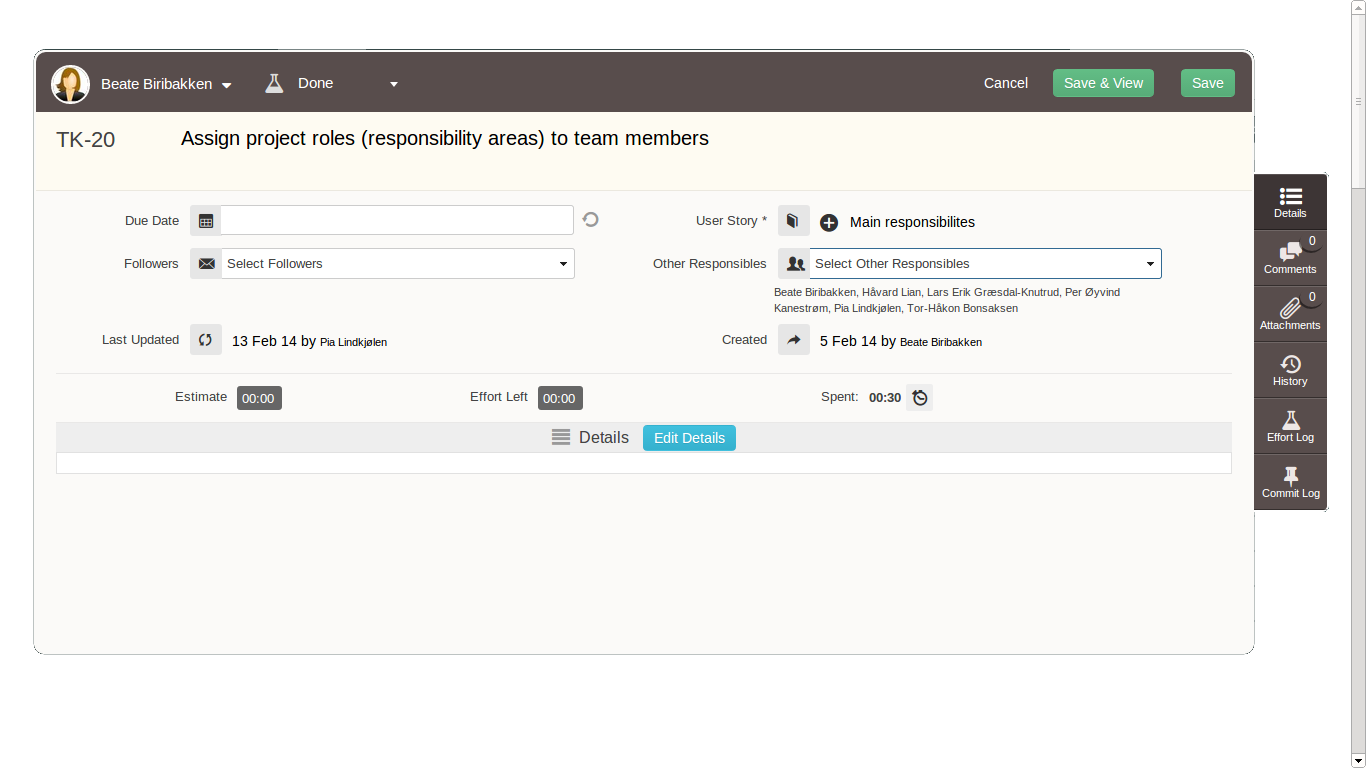
\includegraphics[width=\textwidth]{ch/sprints/fig/wrongUse.png}
\label{fig:wrongUse}
\end{figure}

\begin{figure}[H]
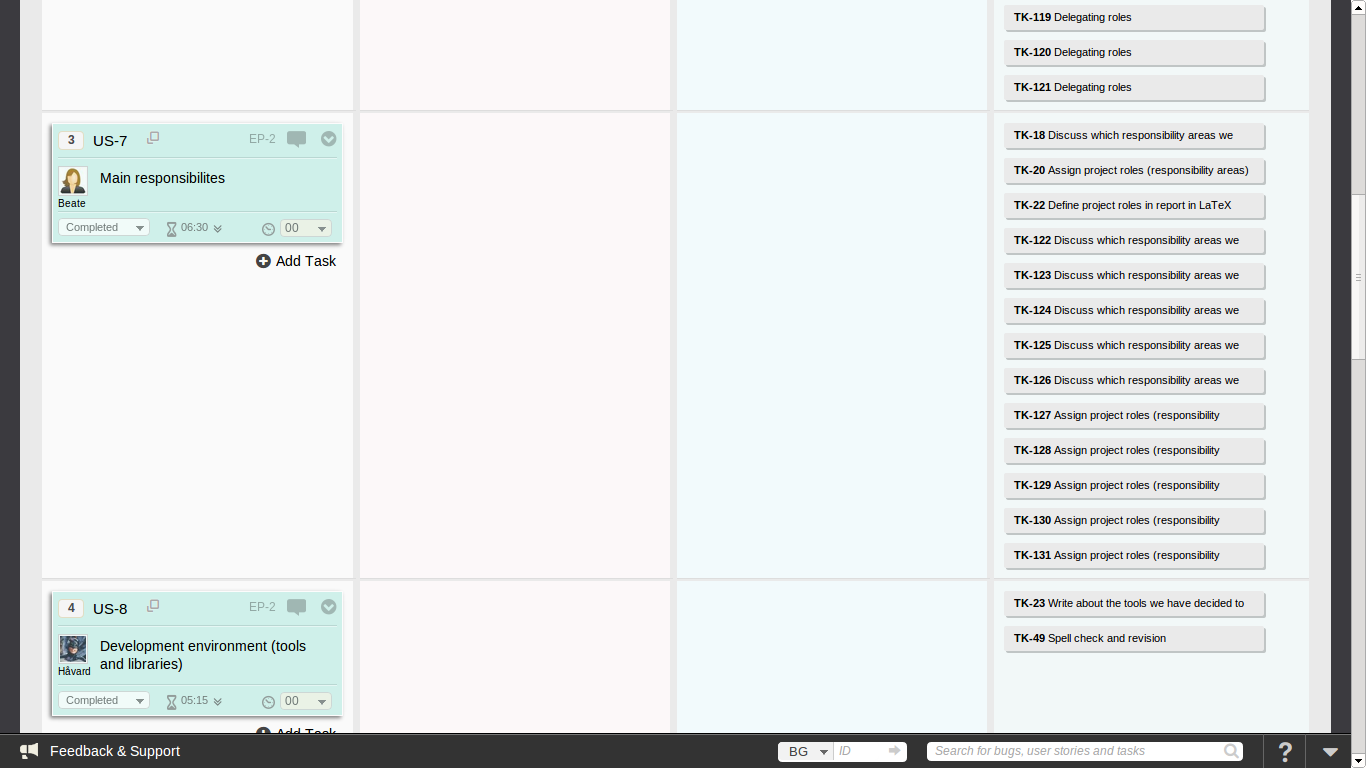
\includegraphics[width=\textwidth]{ch/sprints/fig/addsTasks.png}
\label{fig:addsTasks}
\end{figure}
